\documentclass[a4paper,review,12pt]{elsarticle}

\usepackage[utf8]{inputenc}
\usepackage[T5]{fontenc}
\usepackage{amsmath}
\usepackage{amssymb}
\usepackage{booktabs}
\usepackage{tabularx}
\usepackage{array}
\usepackage{graphicx}
\usepackage{xcolor}
\usepackage{tikz}
\usepackage{pgfplots}
\usepackage{microtype}
\usepackage{xurl}
\usepackage[hidelinks]{hyperref}

\usetikzlibrary{arrows.meta,positioning,shapes.geometric,fit,calc,matrix}
\pgfplotsset{compat=1.18}
\definecolor{paceblue}{HTML}{0072B2}
\definecolor{pacesky}{HTML}{56B4E9}
\definecolor{pacegreen}{HTML}{009E73}
\definecolor{paceorange}{HTML}{E69F00}
\definecolor{pacevermillion}{HTML}{D55E00}
\definecolor{pacepurple}{HTML}{CC79A7}

\journal{Image and Vision Computing}

\newcommand{\method}{PACE-Seg}
\newcommand{\miou}{mIoU}
\newcommand{\etal}{et al.}

\begin{document}

\begin{frontmatter}

\title{PACE-Seg: Hardware-Cost-Conditioned Elastic Semantic Segmentation with Calibrated Risk Routing for Edge Accelerators}

\author{Dũng Nguyễn}

\begin{abstract}
Semantic segmentation on heterogeneous edge accelerators must balance image-dependent prediction difficulty against platform-dependent latency. A fixed model exposes only one operating point, while an elastic network exposes several candidates but does not determine which candidate should process a particular image under a deployment budget. We present \method, an elastic segmentation system with four width--depth--resolution levels and a runtime policy that maps the entropy of one inexpensive probe prediction to a separate expected-error estimate for every candidate. The policy selects the least costly candidate predicted to meet a risk target while enforcing a hard budget using directly measured end-to-end route costs. Calibration is performed separately for each evaluated domain or adverse-condition subset; the experiment therefore assumes that the deployment domain is known or configured and does not evaluate a single condition-agnostic calibrator. We evaluate Cityscapes and the fog, night, rain, and snow subsets of ACDC. A three-run comparison shows that the largest elastic level remains within 1.1 \miou{} points of a similarly sized independently trained Fast-SCNN on every split. Across four edge devices, the evaluated levels span a 110.2-fold FLOPs range but only a 10.3--19.5-fold measured-latency range; a simple proportional FLOPs proxy consequently mis-selects candidates and can violate latency budgets. For the final routing evaluation, we measure complete warm-route latency on a TensorRT/CUDA accelerator and a Hailo-8 dataflow accelerator, then replay held-out per-image predictions with those measured costs. Over three separately trained seed-labelled checkpoints and two backends, the proposed policy outperforms or matches a rank-based calibrated-risk policy in 67 of 69 conditionally fair operating cells (51 wins, 16 ties, and 2 losses), with a macro-averaged gain of 0.0241 \miou{}. It has no budget-violating operating cell among 120 evaluated cells, compared with 51 for the baseline; this zero count is partly a consequence of the hard constraint by design. The two backend evaluations share segmentation predictions, and the operating cells are correlated, so neither count is treated as an independent-sample statistical result. We additionally show that EMA-percentile activation calibration keeps fake-quantized QAT degradation within 1.5 \miou{} points for every tested seed and elasticity level, without claiming compiled INT8 accuracy. The results support hardware-cost-conditioned runtime selection within the evaluated, condition-specific calibration protocol while exposing limitations in uncertainty transfer, rank-dominated budgets, compiled-accuracy validation, and energy measurement.
\end{abstract}

\begin{keyword}
semantic segmentation \sep elastic neural networks \sep dynamic inference \sep uncertainty calibration \sep edge acceleration \sep hardware-aware deployment
\end{keyword}

\end{frontmatter}

\section{Introduction}
\label{sec:introduction}

Semantic segmentation is increasingly deployed on edge systems in autonomous driving, robotics, and augmented reality. Such systems are heterogeneous: two accelerators may assign very different latencies to the same network even when its parameter count and floating-point operation count are unchanged. Prediction quality also varies with the input. Clear daytime images and adverse scenes containing fog, night, rain, or snow need not warrant identical computation. Accuracy alone is therefore insufficient for selecting a deployable segmentation model, and an abstract complexity measure is not a substitute for the route cost observed on the target platform.

Conventional deployment selects one architecture for all inputs. Compact real-time segmentation networks provide useful static speed--accuracy trade-offs, but a single operating point can spend unnecessary computation on easy images and cannot exploit additional budget on harder ones. Training several independent networks creates more operating points but multiplies training, validation, packaging, and maintenance activities. The extent of that overhead is not measured in this work, so we do not claim a quantified reduction in lifecycle cost.

Elastic and slimmable networks address part of this problem by sharing parameters among subnetworks of different capacities. Once trained, one model can expose multiple deployment candidates. Elasticity alone, however, does not specify which candidate should process an image, how uncertainty from a cheap candidate transfers to the others, or how a selection rule should obey an accelerator-specific latency budget. These questions are distinct from producing a set of subnetworks.

Dynamic inference addresses input-dependent computation through gates, early exits, or spatially adaptive routes. Hardware-aware neural architecture search addresses a different axis: it uses measured latency or a latency predictor to select an architecture at design time. \method{} studies their intersection. The available candidates are fixed by an elastic segmentation network; runtime selection is image-dependent; and feasibility is defined by directly measured route costs, including the probe, uncertainty computation, policy, engine dispatch or activation, and any additional candidate inference. This is hardware-cost-conditioned runtime routing, not continuous architecture search and not hardware-aware training.

Uncertainty estimation adds another difficulty. A high-entropy probe prediction may indicate a difficult image, but one scalar does not directly state the expected error of every candidate. A rank-step policy also ignores whether adjacent candidates are separated by one millisecond or tens of milliseconds. We therefore fit, separately within each evaluated domain or condition, a candidate-specific monotonic mapping from a shared probe score to each candidate's observed error and enforce a hard measured-cost budget during selection. The resulting evidence concerns deployments in which the appropriate domain-specific calibration set is known; unknown-condition selection is outside the experiment.

The study asks four bounded questions. First, can measured accelerator cost change candidate selection relative to a simple proportional FLOPs proxy? Second, can a shared elastic network approach the quality of a similarly sized independently trained model? Third, does candidate-specific calibrated routing preserve a favorable quality--latency trade-off after its real route overhead is included? Fourth, can a bounded fake-quant QAT procedure preserve the elastic model's accuracy without being misrepresented as compiled INT8 deployment?

The contributions are as follows:
\begin{enumerate}
    \item We integrate a four-level elastic semantic-segmentation model with per-domain, candidate-specific expected-error calibration from one shared inexpensive probe. Elastic training, sandwich sampling, distillation, and boundary supervision are inherited techniques; the contribution is their use as the candidate family for the measured-budget routing mechanism.
    \item We formulate a runtime policy that selects among those candidates under a hard budget using directly measured end-to-end route costs. This differs from design-time hardware-aware NAS and from rank-only escalation.
    \item We validate route-cost accounting on two structurally different accelerators. TensorRT/CUDA requires accelerator-resident entropy computation to avoid a severe host-side bottleneck, whereas Hailo-8 is dominated by mandatory network-group activation and deactivation.
    \item We provide a bounded empirical analysis of three supporting issues: failure of a simple proportional FLOPs proxy in the evaluated setting, near-parity between the largest elastic level and a matched Fast-SCNN, and the behavior of dynamic, maximum-observer, and EMA-percentile fake-quant QAT.
\end{enumerate}

The claims are intentionally narrower than universal reliability or robustness. The principal routing comparison uses held-out halves of validation splits, offline per-image replay, shared predictions across backends, and correlated operating cells. These boundaries are part of the result rather than post-hoc qualifications.

Figure~\ref{fig:overview} summarizes the complete inference path and separates the shared probe, candidate-specific calibration, measured hardware costs, and hard-budget selection.

\begin{figure*}[t]
\centering
\resizebox{\textwidth}{!}{%
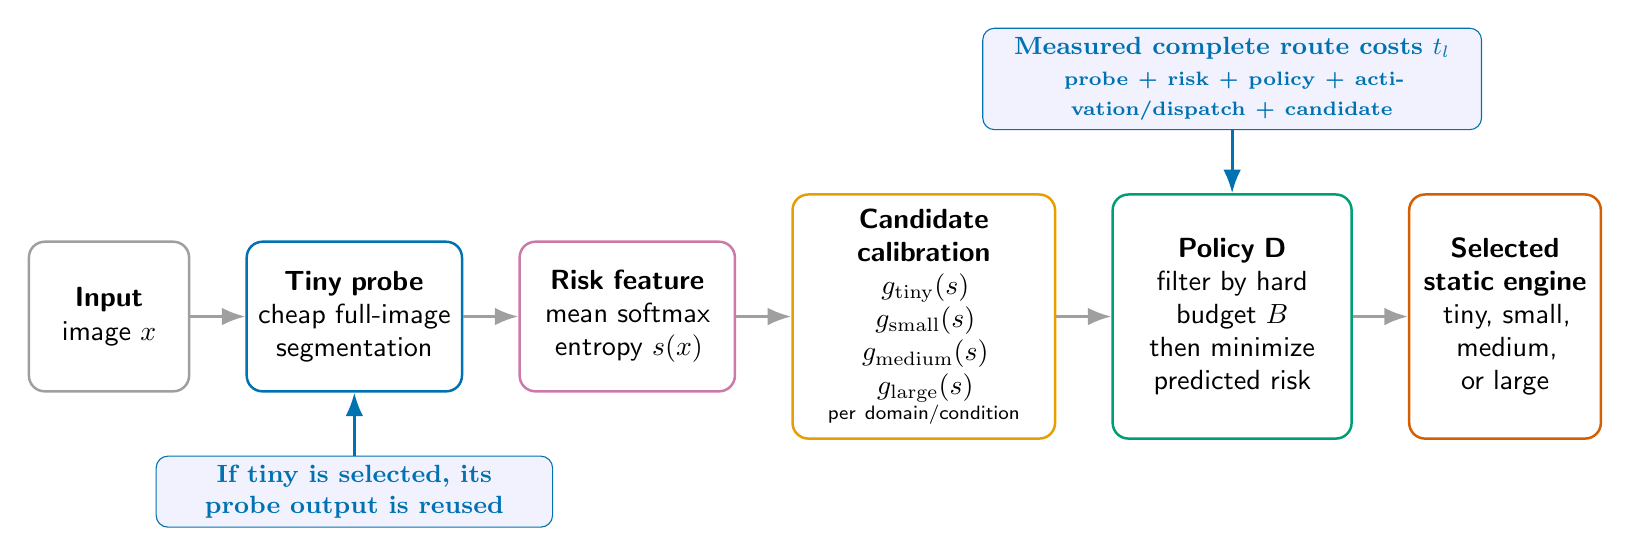
\begin{tikzpicture}[
    font=\sffamily,
    node distance=7mm,
    block/.style={draw, rounded corners=2mm, line width=0.9pt, align=center, minimum height=19mm, text width=25mm, fill=white},
    arrow/.style={-{Latex[length=3mm]}, line width=1pt, draw=gray!75},
    note/.style={draw, rounded corners=1.5mm, align=center, fill=blue!5, draw=paceblue, text=paceblue, font=\bfseries\small}
]
\node[block, draw=gray!75, text width=18mm] (input) {\textbf{Input}\\image $x$};
\node[block, draw=paceblue, right=of input] (probe) {\textbf{Tiny probe}\\cheap full-image segmentation};
\node[block, draw=pacepurple, right=of probe] (entropy) {\textbf{Risk feature}\\mean softmax entropy $s(x)$};
\node[block, draw=paceorange, right=of entropy, text width=31mm, minimum height=31mm] (calib) {\textbf{Candidate calibration}\\$g_{\mathrm{tiny}}(s)$\\$g_{\mathrm{small}}(s)$\\$g_{\mathrm{medium}}(s)$\\$g_{\mathrm{large}}(s)$\\[-1mm]\scriptsize per domain/condition};
\node[block, draw=pacegreen, right=of calib, text width=28mm, minimum height=31mm] (policy) {\textbf{Policy D}\\filter by hard budget $B$\\then minimize predicted risk};
\node[block, draw=pacevermillion, right=of policy, text width=22mm, minimum height=31mm] (engine) {\textbf{Selected static engine}\\tiny, small, medium, or large};

\draw[arrow] (input) -- (probe);
\draw[arrow] (probe) -- (entropy);
\draw[arrow] (entropy) -- (calib);
\draw[arrow] (calib) -- (policy);
\draw[arrow] (policy) -- (engine);

\node[note, above=8mm of policy, text width=61mm] (cost) {Measured complete route costs $t_l$\\\scriptsize probe + risk + policy + activation/dispatch + candidate};
\draw[-{Latex[length=3mm]}, line width=1pt, paceblue] (cost) -- (policy);

\node[note, below=8mm of probe, text width=48mm] (reuse) {If tiny is selected, its probe output is reused};
\draw[-{Latex[length=3mm]}, line width=1pt, paceblue] (reuse) -- (probe);
\end{tikzpicture}%
}
\caption{PACE-Seg inference path. A single tiny prediction supplies the shared entropy feature. Per-domain candidate calibrators estimate each candidate's error, and policy D selects only among candidates feasible under directly measured complete route costs.}
\label{fig:overview}
\end{figure*}


\section{Related work}
\label{sec:related}

\subsection{Efficient and real-time semantic segmentation}

Efficient segmentation research seeks to preserve spatial detail and context while reducing latency. BiSeNet separates spatial and contextual processing~\cite{yu2018bisenet}, STDC removes redundancy from bilateral designs~\cite{fan2021stdc}, and PIDNet adds a boundary-oriented branch to control the interaction between detail and context~\cite{xu2023pidnet}. Transformer-based models such as SegFormer provide another family of accuracy--efficiency operating points~\cite{xie2021segformer}. Collectively, these methods demonstrate that architecture design can substantially improve the static quality--latency trade-off.

The remaining limitation for the present problem is not a lack of compact architectures. A static network commits to one operating point for every image and every budget. Even when several static networks are available, their runtime selection remains external to the architecture. \method{} therefore treats efficient architectures as comparison points and focuses on exposing and selecting multiple capacities within one elastic model.

\subsection{Elastic, slimmable, and once-for-all networks}

Slimmable neural networks introduced shared weights and switchable normalization for execution at multiple widths~\cite{yu2019slimmable}, while universally slimmable networks added the sandwich rule and in-place distillation~\cite{yu2019usnet}. Once-for-All extended the principle across depth, width, kernel size, and resolution and decoupled supernet training from deployment-time specialization~\cite{cai2020ofa}. For semantic segmentation, SlimSeg applied channel slimming, downward distillation, and boundary supervision to produce multiple capacities from one model~\cite{xue2022slimseg}. Multi-Exit Semantic Segmentation Networks pursued a related train-once, customize-at-deployment objective through intermediate exits~\cite{kouris2022mess}.

These works establish that one training process can expose multiple accuracy--efficiency candidates. They do not, by themselves, solve image-wise selection under a hard budget measured on a specific accelerator. OFA-style specialization is primarily deployment-time subnet selection, SlimSeg exposes adjustable widths, and MESS optimizes exit configurations; \method{} instead asks how a shared probe can estimate the error of each available candidate and how those estimates should interact with complete route costs at runtime.

\subsection{Dynamic inference and routing for segmentation}

Dynamic routing for semantic segmentation learns image-dependent paths through a multi-scale network and can regularize expected computation~\cite{li2020dynamic}. Anytime Dense Prediction adds confidence-adaptive exits and spatial masking~\cite{liu2022anytime}, while MESS uses early exits to adapt computation to input difficulty~\cite{kouris2022mess}. These methods show that dense prediction can allocate computation conditionally rather than execute a fixed graph for every input.

\method{} differs in the object being routed and the constraint used. It chooses among separately compiled elastic candidates rather than internal paths or intermediate heads. Its baseline and proposed policies both use one cheap full-image probe, but the proposed policy predicts a distinct error for each candidate and admits only candidates within a measured end-to-end budget. The method is therefore closer to calibrated model selection than to a learned architectural gate. It does not claim end-to-end optimal routing or a formal risk guarantee.

\subsection{Hardware-aware model selection and NAS for segmentation}

Platform-aware NAS established that real latency can be a more faithful objective than FLOPs for mobile deployment~\cite{tan2019mnasnet}. Segmentation-specific systems such as FasterSeg, AutoSegEdge, multi-objective edge NAS, and RealtimeSeg incorporate latency into architecture optimization and deploy searched models on edge hardware~\cite{chen2020fasterseg,dou2023autosegedge,dou2024multiobjective,li2023realtimeseg}. These studies collectively establish that deployment cost should enter model design and that FLOPs alone need not preserve latency ordering or magnitude.

The distinction from \method{} is temporal. Hardware-aware NAS makes design-time decisions about an architecture or search space. \method{} does not feed hardware cost back into supernet training and does not perform continuous architecture search. It performs post-training, runtime selection among four fixed candidates. Its RQ1 claim is correspondingly narrow: in the measured four-candidate setting, a simple through-origin proportional FLOPs proxy can reproduce neither the observed cost scale nor all budget-feasible choices. This does not imply that FLOPs-aware NAS in general is inferior, nor that learned latency predictors cannot transfer.

\subsection{Uncertainty, calibration, and selective segmentation}

Confidence calibration for segmentation is affected by prediction correctness, model capacity, crop size, and domain shift~\cite{wang2023calibrating}. Broader evaluations show that improved in-domain accuracy does not automatically imply calibrated uncertainty under datasets such as ACDC~\cite{dejorge2023reliability}. ACDC itself provides fog, night, rain, and snow scenes and supports uncertainty-aware segmentation through invalid-region annotations and UIoU~\cite{sakaridis2021acdc}. Risk--coverage and rejection metrics provide ways to evaluate whether confidence ranks errors, but they do not automatically convert one model's confidence into another model's expected error.

\method{} uses mean softmax entropy from the tiny candidate as a shared feature and fits one monotonic quantile-binned mapping per candidate and per evaluated domain or condition. The approach is calibration-based routing, not a proof that entropy is universally reliable. It also differs from pixel-wise calibration: the output is one image-level expected-error estimate per candidate. This protocol presumes that the appropriate domain-specific calibrator is known at deployment; a pooled or automatically selected unknown-condition calibrator is not evaluated. ACDC/night produces the weakest probe ranking in our evaluation, and ACDC invalid-region labels are not used to report UIoU. These limits prevent a general reliability claim.

\subsection{Quantization of elastic networks}

Adaptive-bit and elastic quantization methods such as AdaBits and EQ-Net train shared networks that support multiple numerical precisions or quantized subnetworks~\cite{jin2020adabits,xu2023eqnet}. They establish that weight sharing and quantization can be optimized jointly, but they do not make fake-quant evidence equivalent to compiled accelerator accuracy. Quantization is therefore a supporting analysis in this work rather than the central novelty: we compare bounded observer choices for the elastic segmentation model and explicitly stop at simulated fake quantization.

\subsection{Positioning of PACE-Seg}

Prior work has separately demonstrated efficient segmentation, elastic subnetworks, input-adaptive computation, hardware-aware architecture selection, and uncertainty-aware prediction. \method{} inherits elastic training and entropy-based confidence estimation. Its contribution lies in combining a shared probe with per-domain candidate-specific error mappings, enforcing a hard budget defined by measured complete route costs, and auditing the resulting policy on TensorRT/CUDA and Hailo-8. The evidence is deployment-oriented and integrative: it does not establish priority for slimmable segmentation, dynamic routing, calibration, or hardware-aware search as individual ideas, nor does it establish condition-agnostic calibration.

\section{Method}
\label{sec:method}

\subsection{Elastic candidate family}
\label{sec:elastic}

\method{} contains four discrete levels: tiny, small, medium, and large. Their width multipliers are 0.25, 0.50, 0.75, and 1.00; their repeated block counts are 2, 3, 4, and 6; and their input resolutions are $384\times192$, $512\times256$, $768\times384$, and $1024\times512$ pixels. The levels share convolutional weights through active-channel slicing and use level-specific batch-normalization state. The operator set is restricted to convolutions, normalization, standard activations, pooling, elementwise operations, concatenation, and static-factor bilinear resizing that passed compiler smoke tests in the evaluated toolchains. Because no unconstrained-operator control was trained, compiler compatibility is deployment evidence rather than a measured accuracy contribution.

Training uses the sandwich rule: each step evaluates the smallest and largest levels and one randomly selected intermediate level. The largest level receives supervised segmentation loss, smaller levels receive supervised and in-place distillation terms, and a boundary auxiliary term emphasizes semantic transitions. The default run uses 100,000 optimization steps, batch size 8, AdamW with weight decay $10^{-4}$, initial learning rate $3\times10^{-4}$, cosine decay, 500 warm-up steps, and gradient clipping at 5.0. The data stream combines Cityscapes and ACDC with random scale/crop/pad, horizontal flip, and color jitter.

The four levels are exported as separate static graphs. Runtime routing therefore selects an engine before the selected candidate is executed; no compiled graph contains data-dependent control flow.

\subsection{Shared probe and candidate-specific error calibration}
\label{sec:calibration}

Let the tiny candidate produce logits $z(x)$. The raw probe score is mean pixel entropy,
\begin{equation}
s(x)=\frac{1}{|\Omega|}\sum_{u\in\Omega}-\sum_{c=1}^{C}p_{u,c}\log\max(p_{u,c},10^{-12}),
\label{eq:entropy}
\end{equation}
where $p$ is the softmax of $z$ and $C=19$. The score is image-level and requires no separate probe network.

For each candidate $l$, we fit a monotonic calibrator $g_l$ that maps the same $s(x)$ to the candidate's observed per-image pixel error. A separate set of candidate calibrators is fitted for Cityscapes and for each ACDC condition; calibrators are not pooled across the five splits. Fit-half samples are divided into ten equal-count bins by probe score. The target in each bin is the mean observed error of candidate $l$, and a cumulative-maximum pass enforces non-decreasing expected error. Thus
\begin{equation}
\widehat{r}_l(x)=g_l(s(x))
\label{eq:risk}
\end{equation}
is candidate-specific calibration from shared sensing, not candidate-specific probing. At deployment, this formulation requires the relevant domain or condition to be known or otherwise configured so that the corresponding calibrator set is selected.

The implementation computes fit-half entropy only over ground-truth-valid pixels but computes inference and held-out entropy over all pixels because an ignore mask is unavailable at deployment. This does not expose held-out ground truth to the policy, but it is a fit--deployment feature mismatch. We retain the frozen evidence and disclose the mismatch rather than describing the calibrator as perfectly deployment-matched.

\subsection{Hardware-cost-conditioned policy}
\label{sec:policy}

For a target device, candidate $l$ has measured route cost $t_l$, risk target $\tau$, and budget $B$. The proposed policy D forms the feasible set
\begin{equation}
\mathcal{S}_B=\{l:t_l\leq B\}.
\label{eq:feasible}
\end{equation}
If at least one feasible candidate satisfies $\widehat{r}_l(x)\leq\tau$, D selects the cheapest such candidate. Otherwise it selects the feasible candidate with minimum predicted error, breaking ties by lower cost. If no candidate is within budget, it selects the globally cheapest candidate. The final fallback can still exceed a budget smaller than the cheapest available route; the evaluated budget grid uses the four measured route costs, so this case does not occur in the reported final cells.

We compare D with three progressive ablations. A uses one calibrator for the probe candidate and escalates by latency rank according to integer multiples of $\tau$. B retains the single risk value but targets a latency magnitude before choosing the closest candidate. C uses candidate-specific risks but has no explicit budget. The progression is not a factorial $2\times2$ because D adds a hard-budget axis absent from A--C. Static candidates, uncalibrated entropy routing, and a ground-truth oracle are additional references. The oracle is used only as an upper bound and never supplies information to a deployable policy.

\subsection{Fit, selection, and held-out protocol}
\label{sec:split}

Each Cityscapes or ACDC validation split is partitioned by alternating index: even-index images form the fit half and odd-index images form the held-out half. Every candidate is evaluated once per image and its prediction is cached. Within each split, that split's candidate calibrators are fitted only from its fit-half probe scores and candidate errors; there is no cross-condition pooling. Five risk targets are the 10th, 25th, 50th, 75th, and 90th percentiles of fit-half observed error, macro-aggregated across the five splits. One canonical risk grid is generated per training run and reused for both E1 and E3; only the measured cost table changes.

For each budget and policy, the representative risk target is selected using fit-half statistics: among points whose fit-half mean cost does not exceed the budget, choose the highest fit-half \miou{} and break ties by lower cost. If no point is feasible, the cheapest point is marked infeasible. Held-out predictions are read only after this choice. The final overhead replay implements this separation for both A and D. An older progressive-evaluation path selected D's point from held-out values, but those outputs are not used for the canonical final claim.

The oracle chooses, independently for each held-out image, the lowest-ground-truth-error candidate within the budget. It bounds available candidate quality; it is not a deployable policy.

Figure~\ref{fig:protocol} makes the data separation explicit. Calibrator fitting, risk-grid construction, and operating-point selection occur on the fit half; the held-out half is used only after the policy is locked.

\begin{figure*}[t]
\centering
\resizebox{0.96\textwidth}{!}{%
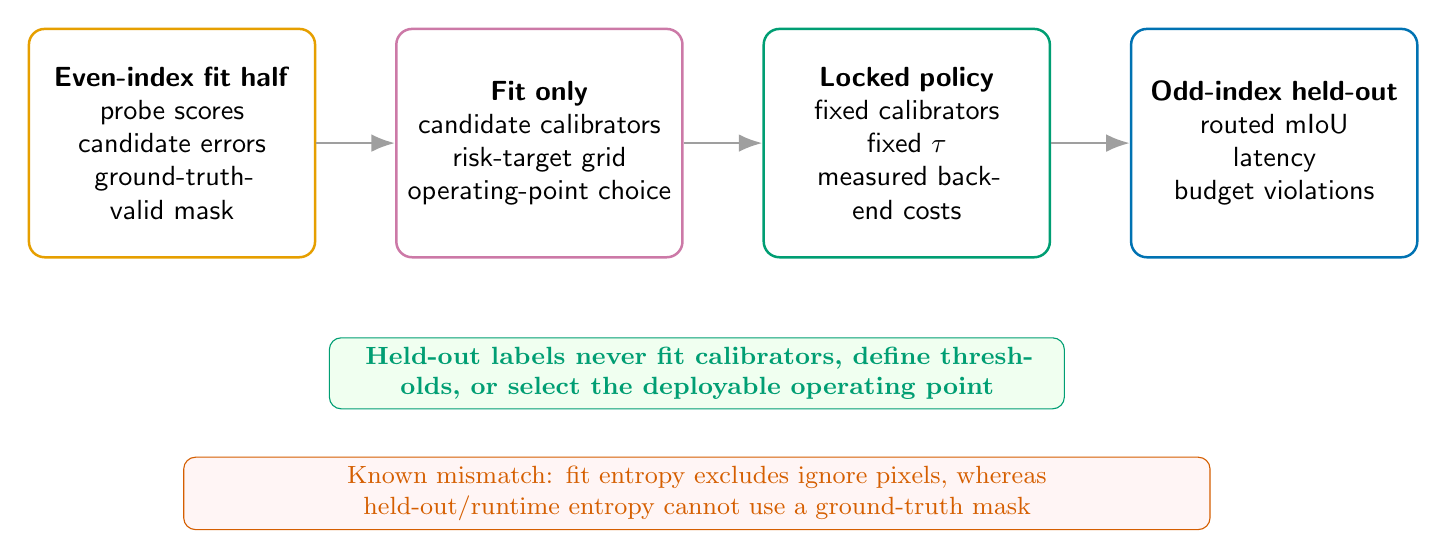
\begin{tikzpicture}[
    font=\sffamily,
    node distance=10mm,
    block/.style={draw, rounded corners=2mm, line width=0.9pt, align=center, minimum height=29mm, text width=34mm, fill=white},
    arrow/.style={-{Latex[length=3mm]}, line width=1pt, draw=gray!75},
    note/.style={draw, rounded corners=1.5mm, align=center, font=\bfseries\small}
]
\node[block, draw=paceorange] (fit) {\textbf{Even-index fit half}\\probe scores\\candidate errors\\ground-truth-valid mask};
\node[block, draw=pacepurple, right=of fit] (fitops) {\textbf{Fit only}\\candidate calibrators\\risk-target grid\\operating-point choice};
\node[block, draw=pacegreen, right=of fitops] (locked) {\textbf{Locked policy}\\fixed calibrators\\fixed $\tau$\\measured backend costs};
\node[block, draw=paceblue, right=of locked] (test) {\textbf{Odd-index held-out}\\routed mIoU\\latency\\budget violations};

\draw[arrow] (fit) -- (fitops);
\draw[arrow] (fitops) -- (locked);
\draw[arrow] (locked) -- (test);

\node[note, below=10mm of fitops, xshift=20mm, text width=91mm, fill=green!6, draw=pacegreen, text=pacegreen] (clean) {Held-out labels never fit calibrators, define thresholds, or select the deployable operating point};
\node[note, below=6mm of clean, text width=128mm, fill=red!4, draw=pacevermillion, text=pacevermillion, font=\small] (mismatch) {Known mismatch: fit entropy excludes ignore pixels, whereas held-out/runtime entropy cannot use a ground-truth mask};
\end{tikzpicture}%
}
\caption{Fit, operating-point selection, and held-out evaluation are separated within every domain or adverse-condition split. The final canonical replay uses the locked fit-half choice; the disclosed ignore-mask mismatch is not held-out label leakage.}
\label{fig:protocol}
\end{figure*}


\subsection{Fake-quantized QAT}
\label{sec:qatmethod}

QAT replaces each convolution with per-tensor symmetric 8-bit fake quantization of its input activation and active weight tensor, using PyTorch's straight-through estimator. Dynamic mode derives the activation scale from every call. Calibrated mode freezes one activation range per layer after a 200-image calibration pass spanning clean and adverse conditions. The original maximum observer retains the largest activation observed over all calls. The final EMA-percentile observer computes the 99.9th percentile of absolute activation in each call and combines successive values with momentum 0.9.

For a slimmable convolution, one calibration buffer belongs to the shared layer and aggregates calls from all elasticity levels; the implementation does not maintain a separate frozen activation scale for each level. Each QAT run fine-tunes 10,000 steps from an FP32 checkpoint at learning rate $3\times10^{-5}$. These are simulated fake-quant results. They neither execute integer kernels nor establish compiled TensorRT or Hailo INT8 accuracy.

\section{Experimental protocol}
\label{sec:protocol}

\subsection{Datasets and metrics}

Cityscapes supplies 2,975 training and 500 validation images~\cite{cordts2016cityscapes}. ACDC supplies 1,600 training and 406 validation images distributed across fog, night, rain, and snow~\cite{sakaridis2021acdc}. Both use the 19 Cityscapes train classes. Segmentation quality is dataset-level mean intersection-over-union. Router calibration targets per-image pixel error, while final routed quality is recomputed by accumulating confusion matrices from the selected candidate and calculating \miou{} once over the routed set.

The main router unit is an operating cell defined by one training run, backend, dataset split, and budget. Cells share images, predictions, thresholds, and often candidate-feasible sets. We therefore report descriptive counts and macro averages without $p$-values or confidence intervals that treat cells as independent samples.

\subsection{Training runs and baselines}

The near-parity comparison uses three augmented supernet runs and three augmented Fast-SCNN runs. The final router package uses the three separately trained seed-labelled checkpoints summarized in Table~\ref{tab:provenance}. Repository naming indicates that two runs are augmentation-labelled and one is the earlier unlabelled configuration; checkpoint hashes, initialization-parent identifiers, and immutable full training manifests are not recorded in the final report. We consequently call them separate training runs rather than a controlled three-seed estimate under a proven identical configuration.

\begin{table}[t]
\centering
\caption{Training-checkpoint provenance used by the final router package. Missing fields are reported rather than inferred.}
\label{tab:provenance}
\small
\begin{tabularx}{\textwidth}{@{}lXclX@{}}
\toprule
Run & Repository experiment ID & Seed & Checkpoint & Provenance boundary \\
\midrule
0 & \texttt{pace\_seg\_v1\_aug\_seed0} & 0 & step 100,000 & Augmentation-labelled ID; checkpoint/config hash and initialization parent unavailable \\
2 & \texttt{pace\_seg\_v1\_seed2} & 2 & step 100,000 & Earlier unlabelled ID; checkpoint/config hash and initialization parent unavailable \\
3 & \texttt{pace\_seg\_v1\_aug\_seed3} & 3 & step 100,000 & Augmentation-labelled ID; checkpoint/config hash and initialization parent unavailable \\
\bottomrule
\end{tabularx}
\end{table}

Fixed-architecture comparisons include Fast-SCNN, BiSeNetV2, SegFormer-B0, DDRNet-23-slim, and MobileNetV3+DeepLabV3. Fast-SCNN is the parameter-matched RQ2 comparator for the large elastic level. Static-small, static-large, raw entropy, rank-based calibrated policy A, latency-spacing policy B, candidate-specific budget-unaware policy C, constrained policy D, and an oracle provide routing references.

\subsection{Device-cost measurement}

Candidate-only latency is measured on four devices: E1, a Raspberry Pi 5 host with a Hailo-8 M.2 accelerator; E2, a Jetson Xavier NX; E3, a Jetson AGX Xavier; and E5, a Jetson Orin Nano. NVIDIA devices use TensorRT FP16. Measurements use batch size one, warm-up, three independent benchmark runs for the candidate lookup table, and bootstrap intervals. Energy is excluded because no external calibrated power meter was available.

The final router claim uses complete warm route costs on E1 and E3. On E3, all four TensorRT contexts are resident. A route measures tiny inference, a GPU-resident entropy kernel, policy computation, context dispatch, and additional selected-candidate inference; tiny output is reused when tiny is selected. On E1, all HEFs are configured but the hardware permits only one active network group, so each inference pays activation and deactivation. Entropy runs on the host because Hailo-8 has no CUDA-like general-purpose kernel path. Each warm route class uses 50 warm-up iterations and at least 500 timed iterations. Cold reload is measured as a stress case but is not used in the final frontier replay because E1 and E3 impose non-equivalent cold semantics.

The route harnesses use compiled graphs with the correct post-rescale architecture but do not execute trained checkpoint weights for the accuracy evaluation. The final result combines measured route latency with cached trained-model predictions in an offline, per-image policy replay. It is not an integrated on-device accuracy run.

\subsection{Fair-cell and violation definitions}

A fair A-versus-D cell is one in which A has zero held-out per-image budget violations at its fit-selected operating point. This conditioning excludes cells where the baseline obtains quality by exceeding its own budget; it does not assert that the remaining 69 cells are random or independent. Because the definition conditions on A's success, it is more favorable to A than pooling its infeasible wins with feasible comparisons. We accompany the fair-cell quality comparison with violation counts over all 120 cells.

An operating cell is called violating when at least one held-out image exceeds the cell's budget. This differs from the mean violation rate within such a cell. D's zero violating-cell count is expected in part because D filters candidates by a hard budget. The empirical question is whether D retains useful quality while satisfying that constraint.

\section{Results}
\label{sec:results}

\subsection{Elastic quality and same-budget near-parity}

The trained levels form a monotonic quality ladder on Cityscapes and every ACDC condition. The headline RQ2 comparison is the large level against an augmented, similarly sized Fast-SCNN. Table~\ref{tab:rq2} reports the three-run means.

\begin{table}[t]
\centering
\caption{Three-run mean \miou{} for the matched RQ2 comparison. Positive gap favors the elastic large level.}
\label{tab:rq2}
\begin{tabular}{@{}lrrr@{}}
\toprule
Split & Fast-SCNN & \method{} large & Gap \\
\midrule
Cityscapes & 0.5228 & 0.5338 & +0.0110 \\
ACDC/fog & 0.5629 & 0.5650 & +0.0021 \\
ACDC/night & 0.3822 & 0.3757 & $-0.0065$ \\
ACDC/rain & 0.5050 & 0.5027 & $-0.0023$ \\
ACDC/snow & 0.5048 & 0.5055 & +0.0007 \\
\bottomrule
\end{tabular}
\end{table}

The elastic level is higher on three splits and lower on two; every absolute difference is at most 0.0110 \miou{}. This supports near-parity, not superiority. It also does not quantify total training or maintenance savings.

\subsection{FLOPs does not reproduce measured cost in this candidate set}

The four levels require 0.2060, 1.1678, 6.1712, and 22.6992 GFLOPs. Their large-to-tiny ratio is 110.2. Measured end-to-end candidate latency grows much less sharply, as shown in Table~\ref{tab:latency}.

\begin{table}[t]
\centering
\caption{Candidate-only mean latency used for the four-device RQ1 analysis.}
\label{tab:latency}
\begin{tabular}{@{}lrrrr@{}}
\toprule
Level & E1 Hailo-8 & E2 Xavier NX & E3 AGX Xavier & E5 Orin Nano \\
\midrule
tiny & 3.714 & 2.061 & 0.912 & 1.081 \\
small & 6.597 & 4.964 & 1.781 & 2.604 \\
medium & 20.29 & 15.10 & 4.546 & 7.727 \\
large & 41.14 & 40.26 & 9.389 & 17.95 \\
\bottomrule
\end{tabular}
\end{table}

Measured large-to-tiny ratios range from 10.3 to 19.5, so the FLOPs ratio overstates cost scaling by roughly 6--11 times. Under a 10~ms budget, measured-cost selection chooses small on E1 and E2, large on E3, and medium on E5. A through-origin proportional FLOPs-to-latency fit calibrated on one device mis-selects at least two of the four targets, with per-level prediction errors reported between 82\% and 365\%. Figure~\ref{fig:flops-latency} visualizes the scale mismatch without implying that every hardware-cost model behaves like this proportional proxy.

\begin{figure}[t]
\centering
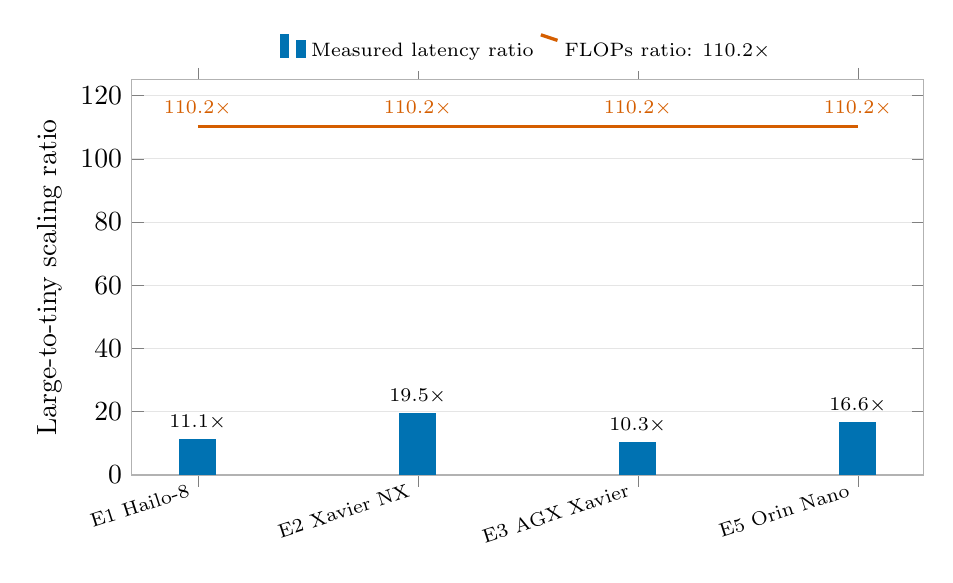
\begin{tikzpicture}
\begin{axis}[
    width=0.96\linewidth,
    height=6.6cm,
    ybar,
    bar width=13pt,
    ymin=0,
    ymax=125,
    ylabel={Large-to-tiny scaling ratio},
    symbolic x coords={E1 Hailo-8,E2 Xavier NX,E3 AGX Xavier,E5 Orin Nano},
    xtick=data,
    x tick label style={rotate=18,anchor=east,font=\scriptsize},
    ymajorgrids=true,
    grid style={gray!20},
    axis line style={gray!60},
    nodes near coords={\pgfmathprintnumber[fixed,precision=1]{\pgfplotspointmeta}$\times$},
    nodes near coords style={font=\scriptsize\bfseries},
    legend style={draw=none,at={(0.5,1.02)},anchor=south,legend columns=2,font=\scriptsize},
]
\addplot[fill=paceblue,draw=paceblue] coordinates {
    (E1 Hailo-8,11.08)
    (E2 Xavier NX,19.53)
    (E3 AGX Xavier,10.30)
    (E5 Orin Nano,16.60)
};
\addlegendentry{Measured latency ratio}
\addplot[pacevermillion,very thick,sharp plot] coordinates {
    (E1 Hailo-8,110.2)
    (E2 Xavier NX,110.2)
    (E3 AGX Xavier,110.2)
    (E5 Orin Nano,110.2)
};
\addlegendentry{FLOPs ratio: $110.2\times$}
\end{axis}
\end{tikzpicture}
\caption{The four candidates span $110.2\times$ in FLOPs but only $10.3$--$19.5\times$ in measured candidate latency. This demonstrates failure of the evaluated proportional FLOPs proxy, not of every FLOPs-aware or learned hardware-cost model.}
\label{fig:flops-latency}
\end{figure}


The broader analysis sweeps 40 log-spaced budgets, four reference devices, and four target devices, producing 640 proxy evaluations. Even same-device proportional fits mis-select 37.5--65\% of budgets. Transfers from faster to slower targets reach 85--95\% mis-selection or violation rates in the worst pairings. The conclusion is limited to this simple proxy, candidate family, and device set. Learned predictors and hardware-aware NAS are not evaluated by this ablation.

\subsection{Progressive routing ablation before complete overhead}

Using candidate-only lookup costs on seed0, D has no violations in 80 device--split--budget cells. A violates 28, B violates 5, C violates 44, and raw entropy violates 20. Among the 52 seed0 cells in which A is feasible, D records 36 wins, 12 ties, and 4 losses, with mean D-minus-A \miou{} of +0.0224. The four losses all correspond to ACDC/rain under one mid-range operating pattern. Candidate-specific calibration inversions average 2.13\%, suggesting that larger candidates are rarely predicted worse than adjacent smaller ones. The raw probe's area under the risk--coverage curve averages 0.1467 and is worst on ACDC/night at 0.2616, showing that uncertainty ranking weakens under the hardest condition.

Replicating the lookup-table comparison on the other two training runs preserved the qualitative advantage, but these pre-overhead values are not the final headline. The next subsection replaces candidate-only lookup costs with measured complete route costs and uses corrected, per-run canonical risk grids.

\subsection{Real route overhead is backend-dependent}

Table~\ref{tab:routes} reports the measured warm route costs used by the final replay. Every row includes the tiny probe and policy path.

\begin{table}[t]
\centering
\caption{Median warm end-to-end route cost used in the final replay.}
\label{tab:routes}
\begin{tabular}{@{}lrr@{}}
\toprule
Route & E3 TensorRT/CUDA & E1 Hailo-8 \\
\midrule
tiny $\rightarrow$ tiny & 2.07 ms & 34.95 ms \\
tiny $\rightarrow$ small & 5.23 ms & 46.13 ms \\
tiny $\rightarrow$ medium & 11.97 ms & 63.36 ms \\
tiny $\rightarrow$ large & 26.70 ms & 92.68 ms \\
\bottomrule
\end{tabular}
\end{table}

On E3, a naive host-side risk path takes approximately 40--80~ms per call and would erase the candidate-latency advantage. A CUDA entropy kernel reduces complete route latency by 2.5--21 times relative to that path. On 40 real TensorRT outputs, 10 per level, its maximum scalar difference from the production PyTorch risk function is $7.15\times10^{-7}$ nats, below the locked $10^{-4}$ tolerance. The tested ten tiny-probe samples produce zero A-policy and zero D-policy decision mismatches. These exact counts establish observed implementation agreement, not a population agreement probability.

On E1, mandatory network-group activation and deactivation dominate. Warm routes are 2--17 times slower than candidate-only streaming values. Cold measurement requires recreating the complete VDevice each iteration because configured groups cannot be individually released and only one VDevice is available. Since this differs from E3's candidate-only reload, cold numbers are reported as backend-specific stress measurements and are not pooled. Figure~\ref{fig:route-overhead} makes the contrast in complete warm-route latency explicit.

\begin{figure}[t]
\centering
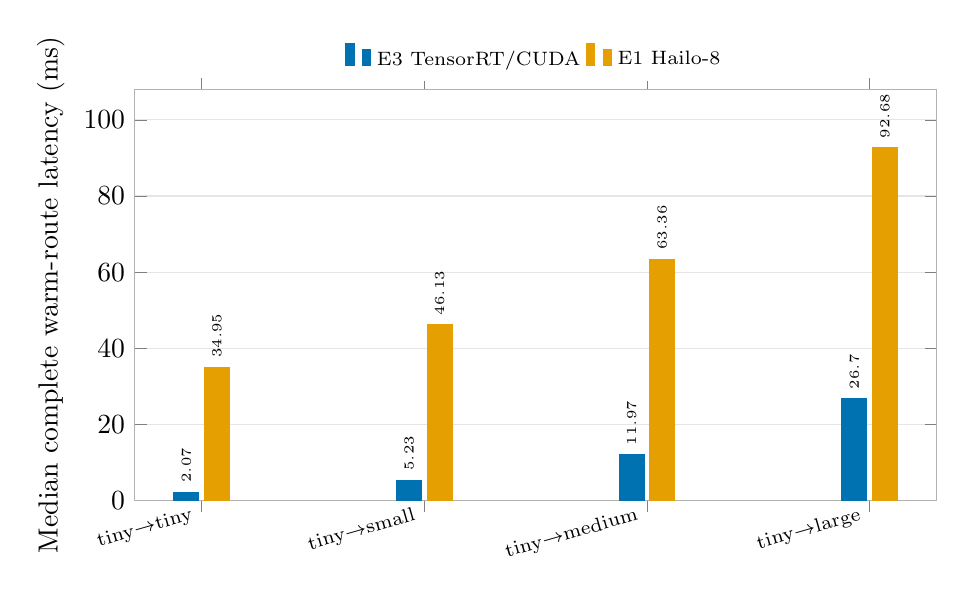
\begin{tikzpicture}
\begin{axis}[
    width=0.97\linewidth,
    height=6.8cm,
    ybar,
    bar width=9pt,
    ymin=0,
    ymax=108,
    ylabel={Median complete warm-route latency (ms)},
    symbolic x coords={tt,ts,tm,tl},
    xtick=data,
    xticklabels={tiny$\rightarrow$tiny,tiny$\rightarrow$small,tiny$\rightarrow$medium,tiny$\rightarrow$large},
    x tick label style={rotate=16,anchor=east,font=\scriptsize},
    ymajorgrids=true,
    grid style={gray!20},
    axis line style={gray!60},
    nodes near coords={\pgfmathprintnumber[fixed,precision=2]{\pgfplotspointmeta}},
    nodes near coords style={font=\tiny,rotate=90,anchor=west},
    legend style={draw=none,at={(0.5,1.02)},anchor=south,legend columns=2,font=\scriptsize},
]
\addplot[fill=paceblue,draw=paceblue] coordinates {
    (tt,2.07)
    (ts,5.23)
    (tm,11.97)
    (tl,26.70)
};
\addlegendentry{E3 TensorRT/CUDA}
\addplot[fill=paceorange,draw=paceorange] coordinates {
    (tt,34.95)
    (ts,46.13)
    (tm,63.36)
    (tl,92.68)
};
\addlegendentry{E1 Hailo-8}
\end{axis}
\end{tikzpicture}
\caption{Complete warm-route costs used in the final replay. E3 requires accelerator-resident entropy computation, while mandatory network-group activation dominates E1. The two backends therefore expose different overhead mechanisms.}
\label{fig:route-overhead}
\end{figure}


\subsection{Canonical overhead-aware router result}

The final replay recomputes A and D decisions with measured warm route costs, constructs the budget grid from the four route costs of each backend, and chooses risk targets from fit-half performance. The same per-run risk grid is used for E1 and E3. Each dataset split retains the calibrators fitted on its own fit half, so these results evaluate condition-specific calibration rather than a single policy that infers an unknown condition.

\begin{table}[t]
\centering
\caption{Final A-versus-D result with measured complete route costs. W/T/L is computed only on fair cells; violations use all cells.}
\label{tab:routerfinal}
\small
\begin{tabular}{@{}lrrrrrr@{}}
\toprule
Backend & Fair & D W/T/L & Win/tie & Macro $\Delta$\miou{} & D viol. & A viol. \\
\midrule
E3 TensorRT/CUDA & 35/60 & 26/8/1 & 97.1\% & +0.0241 & 0/60 & 25/60 \\
E1 Hailo-8 & 34/60 & 25/8/1 & 97.1\% & +0.0241 & 0/60 & 26/60 \\
Overall & 69/120 & 51/16/2 & 97.1\% & +0.0241 & 0/120 & 51/120 \\
\bottomrule
\end{tabular}
\end{table}

D outperforms or matches A in 67 of 69 fair cells. The macro gain of 0.0241 \miou{} equals 2.41 points on the 0--100 scale. This is a descriptive macro average across the three training runs and two cost tables, not an estimate from 69 independent trials. E1 and E3 reuse the same checkpoint predictions; the cross-backend evidence shows that two very different measured cost mechanisms preserve the policy's qualitative advantage, not independent accuracy replication.

The two losses occur in correlated ACDC/rain cells and do not establish a backend-specific failure rate. Identical decisions across backends are also possible when both policies depend on the ordering of four candidates and the budget grid uses those same four breakpoints. Seed2 is an example: backend results coincide despite very different absolute latencies. Seed3 differs by one fair cell because fit-half mean latency crosses a budget boundary differently. Thus hardware costs condition feasibility and deployed latency, but they do not guarantee that every device chooses a different level.

D's 0/120 violation count follows partly from restricting choices to candidates within budget. The substantive result is the quality retained under that constraint and the contrast with A, whose fit-selected rank heuristic creates 51 violating cells. Because fair cells are defined by A's feasibility, the 67/69 quality statement must always be reported with the all-cell violation counts. Figure~\ref{fig:router-result} therefore places the conditional W/T/L comparison beside the full-grid violation counts.

\begin{figure*}[t]
\centering
\begin{minipage}[t]{0.57\textwidth}
\centering
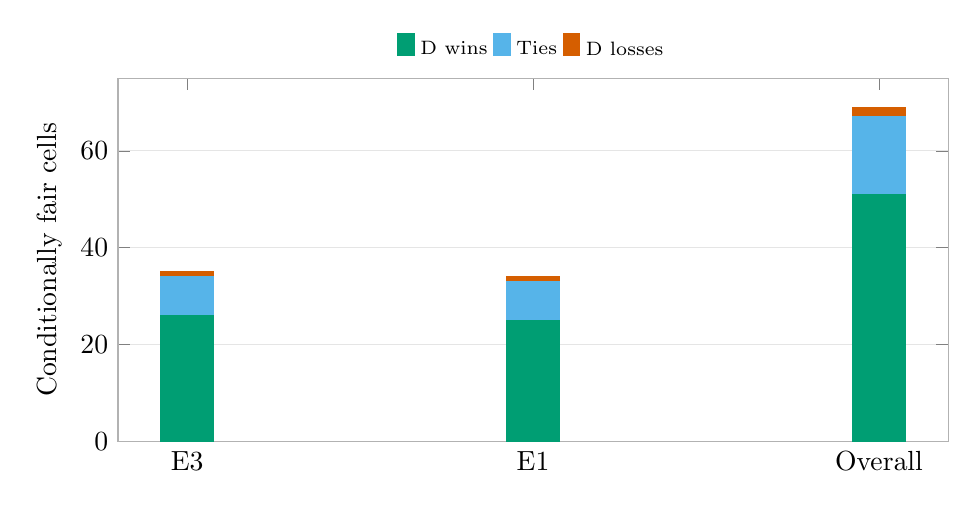
\begin{tikzpicture}
\begin{axis}[
    width=\linewidth,
    height=6.2cm,
    ybar stacked,
    bar width=19pt,
    ymin=0,
    ymax=75,
    ylabel={Conditionally fair cells},
    symbolic x coords={E3,E1,Overall},
    xtick=data,
    ymajorgrids=true,
    grid style={gray!20},
    axis line style={gray!60},
    legend style={draw=none,at={(0.5,1.02)},anchor=south,legend columns=3,font=\scriptsize},
]
\addplot[fill=pacegreen,draw=pacegreen] coordinates {(E3,26) (E1,25) (Overall,51)};
\addlegendentry{D wins}
\addplot[fill=pacesky,draw=pacesky] coordinates {(E3,8) (E1,8) (Overall,16)};
\addlegendentry{Ties}
\addplot[fill=pacevermillion,draw=pacevermillion] coordinates {(E3,1) (E1,1) (Overall,2)};
\addlegendentry{D losses}
\end{axis}
\end{tikzpicture}
\end{minipage}\hfill
\begin{minipage}[t]{0.39\textwidth}
\centering
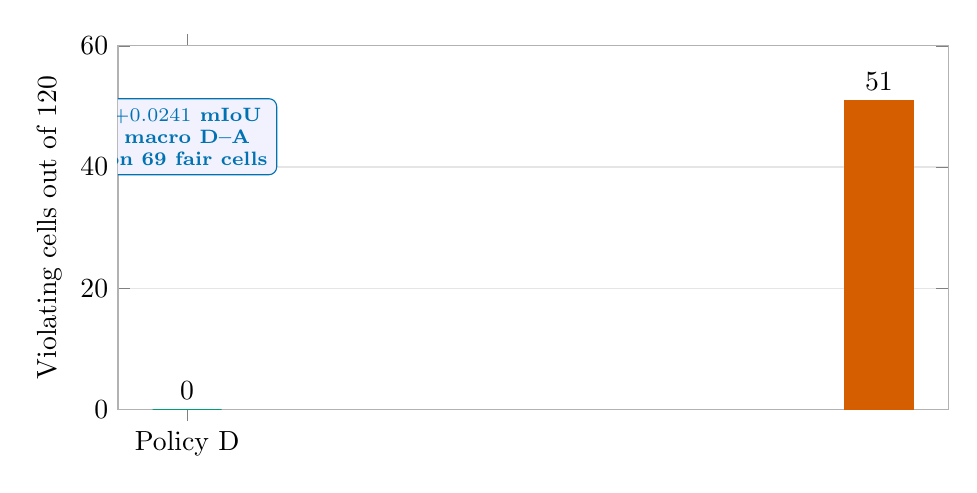
\begin{tikzpicture}
\begin{axis}[
    width=\linewidth,
    height=6.2cm,
    ybar,
    bar width=25pt,
    ymin=0,
    ymax=60,
    ylabel={Violating cells out of 120},
    symbolic x coords={Policy D,Policy A},
    xtick=data,
    ymajorgrids=true,
    grid style={gray!20},
    axis line style={gray!60},
    nodes near coords,
    nodes near coords style={font=\bfseries},
]
\addplot[fill=pacegreen,draw=pacegreen,bar shift=0pt] coordinates {(Policy D,0)};
\addplot[fill=pacevermillion,draw=pacevermillion,bar shift=0pt] coordinates {(Policy A,51)};
\node[align=center,draw=paceblue,fill=blue!5,rounded corners=1mm,text=paceblue,font=\bfseries\scriptsize] at (axis cs:Policy D,45) {$+0.0241$ mIoU\\macro D--A\\on 69 fair cells};
\end{axis}
\end{tikzpicture}
\end{minipage}
\caption{Canonical overhead-aware routing result. Left: D wins or ties in 67 of 69 fair cells (51 wins, 16 ties, 2 losses). Right: across all 120 correlated cells, D has 0 budget-violating cells and A has 51; D's zero count is partly structural because it enforces a hard budget.}
\label{fig:router-result}
\end{figure*}


\subsection{EMA-percentile fake-quant QAT}
\label{sec:qatresults}

Dynamic fake quantization of the shared large level has worst-condition losses of 1.66, 2.54, and 1.39 \miou{} points for the three tested runs, and two runs exceed the predeclared 1.5-point upper bar. Maximum-observer calibration makes seed0 worse on every split. The $2\times2$ seed0 screen shows that changing to EMA-percentile calibration improves worst-condition degradation more than exporting the subnet, while mean effects are not uniformly positive. Because the maximum over conditions can change identity between cells, these differences are not interpreted as additive factorial causal effects.

\begin{table}[t]
\centering
\caption{Absolute worst-condition \miou{} degradation under shared-supernet EMA-percentile fake-quant QAT.}
\label{tab:qat}
\begin{tabular}{@{}lrrrr@{}}
\toprule
Training run & tiny & small & medium & large \\
\midrule
seed-labelled run 0 & 0.32 & 0.97 & 0.51 & 0.97 \\
seed-labelled run 3 & 0.36 & 0.33 & 0.56 & 0.86 \\
seed-labelled run 2 & 0.69 & 0.33 & 0.49 & 1.38 \\
\bottomrule
\end{tabular}
\end{table}

Every evaluated run and level remains within 1.5 points. On the previously worst large-level run, the bound improves from 2.54 to 1.38 points. The supported statement is that this observer stabilizes worst-condition fake-quant degradation in the tested setting. Mean quality is not consistently improved, activation outlier suppression is a plausible but unmeasured mechanism, and compiled INT8 accuracy is unknown. Figure~\ref{fig:qat-heatmap} shows the complete run-by-level worst-condition matrix.

\begin{figure}[t]
\centering
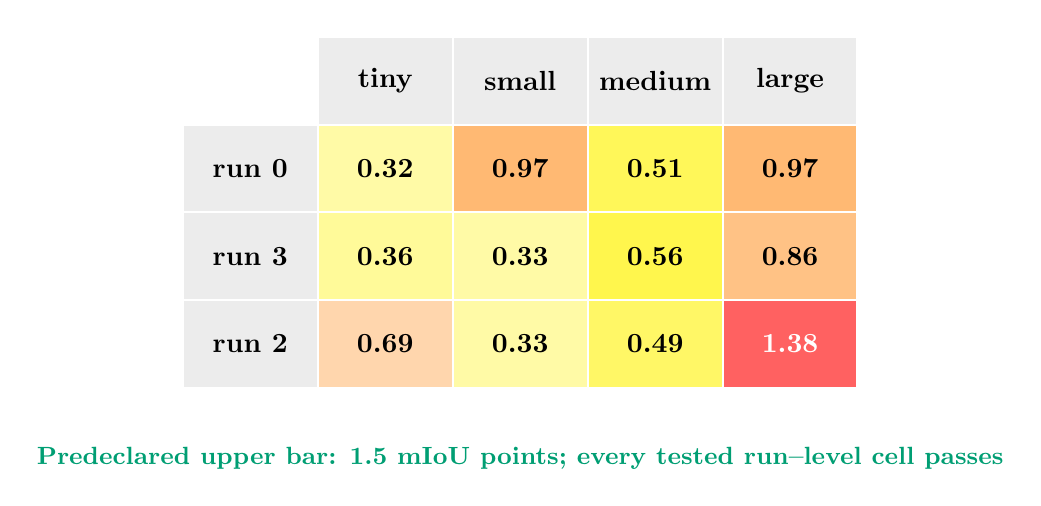
\begin{tikzpicture}[font=\sffamily]
\matrix (m) [matrix of nodes,
    nodes={minimum width=17mm,minimum height=11mm,draw=white,anchor=center,font=\bfseries},
    column sep=0pt,row sep=0pt,
    row 1/.style={nodes={fill=gray!15,font=\bfseries}},
    column 1/.style={nodes={fill=gray!15,font=\bfseries}}
] {
 & tiny & small & medium & large \\
run 0 & |[fill=yellow!35]| 0.32 & |[fill=orange!55]| 0.97 & |[fill=yellow!65]| 0.51 & |[fill=orange!55]| 0.97 \\
run 3 & |[fill=yellow!40]| 0.36 & |[fill=yellow!35]| 0.33 & |[fill=yellow!70]| 0.56 & |[fill=orange!48]| 0.86 \\
run 2 & |[fill=orange!32]| 0.69 & |[fill=yellow!35]| 0.33 & |[fill=yellow!60]| 0.49 & |[fill=red!62,text=white]| 1.38 \\
};
\node[below=5mm of m,align=center,text=pacegreen,font=\bfseries\small] {Predeclared upper bar: 1.5 mIoU points; every tested run--level cell passes};
\end{tikzpicture}
\caption{Absolute worst-condition mIoU degradation after shared-supernet EMA-percentile fake-quant QAT. These are simulated fake-quant results, not compiled INT8 deployment accuracy.}
\label{fig:qat-heatmap}
\end{figure}


\section{Discussion}
\label{sec:discussion}

The results separate three decisions that are often conflated. Elastic training determines which candidates exist. Hardware measurement determines their cost and the feasible set under a deployment budget. Calibrated routing decides which feasible candidate should process an image. \method{}'s strongest evidence concerns the third decision after the second is measured directly.

The FLOPs experiment explains why the separation matters. FLOPs correctly orders the four levels here but badly exaggerates spacing and cannot reproduce all device-specific budget choices. D does not require a globally accurate latency model; it needs a small measured table of complete route costs. This simplicity is useful for four candidates, although it would become costly for a much larger architecture space.

Within each evaluated domain or condition, candidate-specific calibration improves on a single probe-to-rank heuristic because the same entropy can imply different expected errors for different candidates. The low inversion rate indicates that the mappings generally preserve the expected quality ordering. Yet the high AURC on ACDC/night shows that calibration cannot create information absent from the probe. Moreover, selecting the appropriate per-condition calibrator is assumed rather than learned. A pooled calibrator, an explicit condition detector, a richer score, or temporal evidence may relax that assumption, but none is evaluated here.

The overhead study changes the interpretation of hardware-aware routing. On E3, moving uncertainty computation to the accelerator is necessary; on E1, that optimization is unavailable and engine activation dominates. A candidate-only lookup table therefore omits costs that are both large and architecture-dependent. Measuring a route as one trace avoids double-counting and exposes these mechanisms.

The QAT study provides a cautionary parallel. The initial dynamic method and maximum observer support different conclusions from the final EMA-percentile observer. Reporting only an average would have hidden large adverse-condition degradation, while calling the result INT8 deployment would have confused simulated quantization with a compiled engine. The final claim is consequently secondary and explicitly limited to fake quantization.

\section{Limitations and threats to validity}
\label{sec:limitations}

First, calibration is domain- and condition-specific. Cityscapes and each ACDC condition use calibrators fitted on their own fit halves. The evaluation therefore assumes that the deployment domain or adverse condition is known or configured; it does not demonstrate a pooled calibrator or automatic selection under an unknown condition. The router calibration feature also differs between fitting and deployment: fit-half entropy excludes ground-truth ignore pixels, whereas held-out and runtime entropy include all pixels. Held-out labels do not enter policy selection, so this is not test-label leakage, but it is a supervised feature mismatch that may shift calibrator bins. A fully deployment-matched rerun should compute both fit and inference entropy without the ignore mask.

Second, the evaluation uses alternating halves of validation splits rather than an external test set. Multiple budgets and thresholds reuse the same images and predictions. Operating cells are therefore correlated, and the 120-cell denominator is not a statistical sample size. The three checkpoint runs are the main training-replication axis, but complete immutable training provenance, checkpoint hashes, initialization parents, and proof of identical configurations are incomplete.

Third, fair-cell conditioning is descriptive. It excludes A's budget-violating comparisons so quality is compared only when A honors its contract, but the denominator depends on baseline behavior. The full-grid violation counts are required beside the 67/69 result. D's zero violations are partly guaranteed by construction and should not be interpreted as empirical reliability.

Fourth, E1 and E3 share segmentation predictions. The hardware evidence consists of separately measured complete route-cost tables combined with the same per-image prediction caches. Compiled engines used for timing have the correct architecture but are not the trained engines used to produce accuracy. The study therefore validates cost accounting and overhead-aware replay, not bit-exact compiled-model accuracy or a continuously running integrated application.

Fifth, breakpoint budgets can reduce hardware conditioning to latency rank. Absolute costs change feasibility and mean-latency operating-point selection, but identical orderings can produce identical route choices. The term hardware-cost-conditioned describes the policy input; it does not imply that decisions must differ across devices.

Sixth, QAT uses shared per-layer calibration buffers across levels and fake quantization in PyTorch. No compiled INT8 accuracy, integer-kernel speedup, or backend-specific quantization behavior is established. The observed advantage of EMA-percentile calibration is consistent with reduced outlier sensitivity but does not measure activation distributions directly.

Seventh, no external power meter was available, so the paper makes no energy claim. DLA executes only the encoder because of a 16-subgraph hardware limit and is not a headline backend. Temporal-window routing, UIoU, cold-frontier replay, and a decomposition of E3's naive host risk path remain future work. ACDC/night's weak probe signal is an observed limitation, not evidence of universal adverse-condition robustness.

Finally, the supernet's compiler-safe operator set was smoke-tested but not compared with a trained unconstrained search space. Compiler portability should therefore be read as an engineering constraint and validation outcome, not an independently demonstrated algorithmic contribution.

\section{Conclusion}
\label{sec:conclusion}

\method{} combines an elastic segmentation model with per-domain candidate-specific calibration and measured-budget runtime routing. In the evaluated four-candidate system, measured accelerator latency differs substantially from a simple proportional FLOPs proxy, while the largest elastic level remains near a matched independently trained model across clean and adverse conditions. After complete warm route costs are measured on TensorRT/CUDA and Hailo-8, offline per-image replay shows that the constrained candidate-specific policy outperforms or matches the rank baseline in 67 of 69 fair cells, gains 0.0241 \miou{} on average, and satisfies every evaluated budget where the rank baseline creates 51 violating cells. These counts are correlated, the backends share predictions, zero violations partly follow from the policy design, and each condition uses its own fit-half calibrators. The study therefore supports a bounded conclusion: directly measured route costs and candidate-specific error calibration can improve runtime selection among elastic segmentation candidates when the deployment domain is known, but they do not establish condition-agnostic routing, universal reliability, compiled INT8 accuracy, energy savings, or independent cross-device accuracy replication.

\section*{Data and code availability}

The repository records the implementation, experiment reports, and canonical result artifacts. The immutable authoring snapshot used for this manuscript is commit \texttt{ac65b562ed1cc33b7a30a63b2451924b156f8bdd}; the evidence package identified inside that snapshot is based on commit \texttt{1c4d42a7ea525931154ebb2f9015d898ef7771a5}. The final overhead-aware router evidence is stored in \path{reports/router_overhead_replay_E3_20260922.json}, \path{reports/router_overhead_replay_E1_20260928.json}, the corresponding seed2 and seed3 E1/E3 replay files dated 2026-09-29, \path{reports/router_overhead_v1_20260922.md}, and \path{reports/audit_gpu_risk_kernel_production_E3.json}. Dataset access remains subject to the Cityscapes and ACDC licenses.

\begin{thebibliography}{99}

\bibitem{yu2018bisenet}
C. Yu, J. Wang, C. Peng, C. Gao, G. Yu, N. Sang,
BiSeNet: Bilateral segmentation network for real-time semantic segmentation,
in: European Conference on Computer Vision, 2018, pp. 325--341.
\url{https://openaccess.thecvf.com/content_ECCV_2018/html/Changqian_Yu_BiSeNet_Bilateral_Segmentation_ECCV_2018_paper.html}.

\bibitem{fan2021stdc}
M. Fan, S. Lai, J. Huang, X. Wei, Z. Chai, J. Luo, X. Wei,
Rethinking BiSeNet for real-time semantic segmentation,
in: IEEE/CVF Conference on Computer Vision and Pattern Recognition, 2021, pp. 9716--9725.
\url{https://openaccess.thecvf.com/content/CVPR2021/html/Fan_Rethinking_BiSeNet_for_Real-Time_Semantic_Segmentation_CVPR_2021_paper.html}.

\bibitem{xu2023pidnet}
J. Xu, Z. Xiong, S.P. Bhattacharyya,
PIDNet: A real-time semantic segmentation network inspired by PID controllers,
in: IEEE/CVF Conference on Computer Vision and Pattern Recognition, 2023, pp. 19529--19539.
\url{https://openaccess.thecvf.com/content/CVPR2023/html/Xu_PIDNet_A_Real-Time_Semantic_Segmentation_Network_Inspired_by_PID_Controllers_CVPR_2023_paper.html}.

\bibitem{xie2021segformer}
E. Xie, W. Wang, Z. Yu, A. Anandkumar, J.M. Alvarez, P. Luo,
SegFormer: Simple and efficient design for semantic segmentation with transformers,
Advances in Neural Information Processing Systems 34 (2021) 12077--12090.

\bibitem{yu2019slimmable}
J. Yu, L. Yang, N. Xu, J. Yang, T. Huang,
Slimmable neural networks,
in: ICLR Workshop, 2019.
\url{https://arxiv.org/abs/1812.08928}.

\bibitem{yu2019usnet}
J. Yu, T. Huang,
Universally slimmable networks and improved training techniques,
in: IEEE/CVF International Conference on Computer Vision, 2019, pp. 1803--1811.
\url{https://doi.org/10.1109/ICCV.2019.00189}.

\bibitem{cai2020ofa}
H. Cai, C. Gan, T. Wang, Z. Zhang, S. Han,
Once-for-All: Train one network and specialize it for efficient deployment,
in: International Conference on Learning Representations, 2020.
\url{https://openreview.net/forum?id=HylxE1HKwS}.

\bibitem{xue2022slimseg}
D. Xue, F. Yang, P. Wang, L. Herranz, J. Sun, Y. Zhu, Y. Zhang,
SlimSeg: Slimmable semantic segmentation with boundary supervision,
in: Proceedings of the 30th ACM International Conference on Multimedia, 2022, pp. 6539--6548.
\url{https://doi.org/10.1145/3503161.3548191}.

\bibitem{kouris2022mess}
A. Kouris, S.I. Venieris, S. Laskaridis, N.D. Lane,
Multi-exit semantic segmentation networks,
in: European Conference on Computer Vision, 2022, pp. 330--349.

\bibitem{li2020dynamic}
Y. Li, L. Song, Y. Chen, Z. Li, X. Zhang, X. Wang, J. Sun,
Learning dynamic routing for semantic segmentation,
in: IEEE/CVF Conference on Computer Vision and Pattern Recognition, 2020, pp. 8553--8562.

\bibitem{liu2022anytime}
Z. Liu, Z. Xu, H.-J. Wang, T. Darrell, E. Shelhamer,
Anytime dense prediction with confidence adaptivity,
in: International Conference on Learning Representations, 2022.
\url{https://openreview.net/forum?id=kNKFOXleuC}.

\bibitem{tan2019mnasnet}
M. Tan, B. Chen, R. Pang, V. Vasudevan, M. Sandler, A. Howard, Q.V. Le,
MnasNet: Platform-aware neural architecture search for mobile,
in: IEEE/CVF Conference on Computer Vision and Pattern Recognition, 2019, pp. 2820--2828.

\bibitem{chen2020fasterseg}
W. Chen, X. Gong, X. Liu, Q. Zhang, Y. Li, Z. Wang,
FasterSeg: Searching for faster real-time semantic segmentation,
in: International Conference on Learning Representations, 2020.
\url{https://openreview.net/forum?id=BJgqQ6NYvB}.

\bibitem{dou2023autosegedge}
Z. Dou, D.-Y. Ye, B. Wang, X. Wang, S. Sun,
AutoSegEdge: Searching for the edge device real-time semantic segmentation based on multi-task learning,
Image and Vision Computing 136 (2023) 104719.
\url{https://doi.org/10.1016/j.imavis.2023.104719}.

\bibitem{dou2024multiobjective}
Z. Dou, D.-Y. Ye, B. Wang, X. Wang, S. Sun,
Multi-objective neural architecture search for efficient and fast semantic segmentation on edge,
IEEE Transactions on Intelligent Vehicles 9 (1) (2024) 1346--1357.
\url{https://doi.org/10.1109/TIV.2023.3332594}.

\bibitem{li2023realtimeseg}
Y. Li, C. Yang, P. Zhao, G. Yuan, W. Niu, J. Guan, H. Tang, M. Qin, Q. Jin, B. Ren, X. Lin, Y. Wang,
Towards real-time segmentation on the edge,
Proceedings of the AAAI Conference on Artificial Intelligence 37 (2) (2023) 1339--1347.
\url{https://doi.org/10.1609/aaai.v37i2.25232}.

\bibitem{wang2023calibrating}
D. Wang, B. Gong, L. Wang,
On calibrating semantic segmentation models: Analyses and an algorithm,
in: IEEE/CVF Conference on Computer Vision and Pattern Recognition, 2023, pp. 23652--23662.

\bibitem{dejorge2023reliability}
P. de Jorge, R. Volpi, P.H.S. Torr, G. Rogez,
Reliability in semantic segmentation: Are we on the right track?,
in: IEEE/CVF Conference on Computer Vision and Pattern Recognition, 2023, pp. 2456--2465.

\bibitem{sakaridis2021acdc}
C. Sakaridis, D. Dai, L. Van Gool,
ACDC: The adverse conditions dataset with correspondences for semantic driving scene understanding,
in: IEEE/CVF International Conference on Computer Vision, 2021, pp. 10765--10775.

\bibitem{cordts2016cityscapes}
M. Cordts, M. Omran, S. Ramos, T. Rehfeld, M. Enzweiler, R. Benenson, U. Franke, S. Roth, B. Schiele,
The Cityscapes dataset for semantic urban scene understanding,
in: IEEE Conference on Computer Vision and Pattern Recognition, 2016, pp. 3213--3223.

\bibitem{xu2023eqnet}
S. Xu, Y. Li, M. Lin, P. Gao, G. Guo, J. Lue, B. Zhang,
EQ-Net: Elastic quantization neural networks,
in: IEEE/CVF International Conference on Computer Vision, 2023, pp. 15072--15082.

\bibitem{jin2020adabits}
Q. Jin, L. Yang, Z. Liao,
AdaBits: Neural network quantization with adaptive bit-widths,
in: IEEE/CVF Conference on Computer Vision and Pattern Recognition, 2020, pp. 2146--2156.

\end{thebibliography}

\end{document}
